\section{GRATiS Design}\label{sec:gratis-design}

\subsection{Offline vs. on-the-fly model exploration}
The exploration of the graph grammar can be done in two ways: \textit{on the fly}, rule transitions are explored only when chosen by the Test Manager, or \textit{offline}, the graph grammar is transformed to an STS and sent to the Test Manager.

On-the-fly model exploration does not encounter the reachability problems discussed in the previous section. However, coverage statistics cannot be calculated on GRATiS, if the model exploration is done on the fly. The number of states/locations and transitions/switch relations the model has when completely explored are not known, so a percentage cannot be derived. As coverage statistics are an important metric, the offline model exploration is chosen for GRATiS.

\subsection{Tool architecture}
GRATiS uses GROOVE as a replacement of the STS in ATM. Figure~\ref{fig:tooling} shows this graphically. GROOVE has several exploration strategies for exploring a graph grammar. A new strategy is added, the \textit{symbolic exploration strategy}. This strategy transforms the graph states and rule transitions found to an STS, following the transformation rules in section~\ref{sec:gg-to-sts}.

The interface on the GROOVE side is implemented by means of a \textit{remote exploration strategy}. This strategy uses the symbolic exploration strategy to derive an STS and sends an HTTP POST request with the STS formatted as JSON to the ATM interface.

The ATM interface receives the HTTP request, parses the JSON to an STS, starts the STS Engine with the STS and initiates the test run.

\begin{figure}[ht]
  \begin{center}
    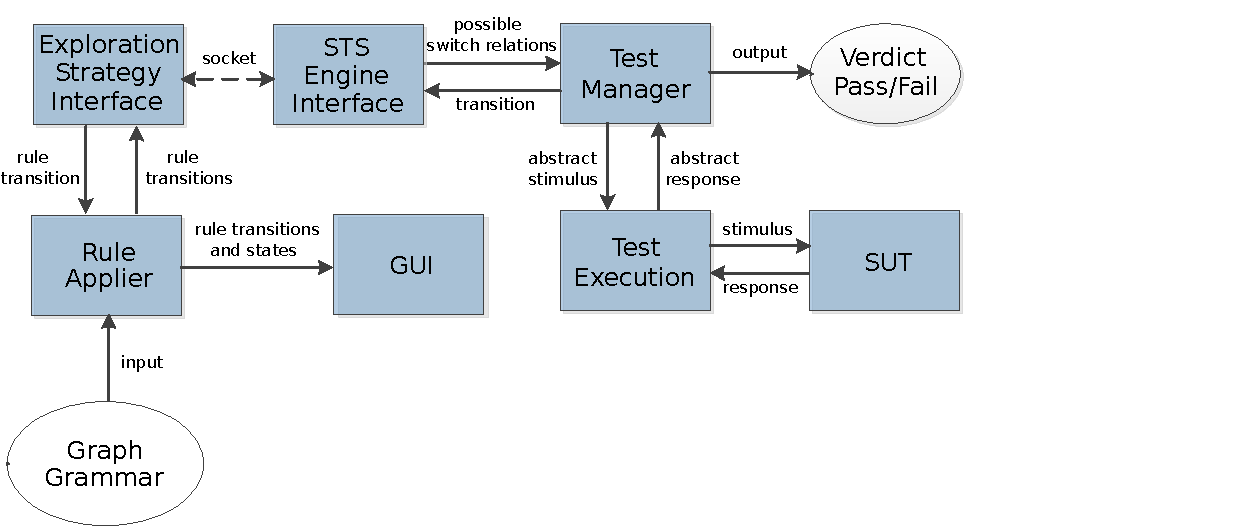
\includegraphics[width=\textwidth]{tooling.pdf}
  \end{center}
  \caption{The GRATiS design: replacing the STS with GROOVE}
  \label{fig:tooling}
\end{figure}
